% Compile with LuaLaTeX, BibTeX, and two further LuaLaTeX passes.
\documentclass[11pt]{article}
\usepackage{acl}
\usepackage{fontspec}
\IfFontExistsTF{TeX Gyre Termes}{\setmainfont{TeX Gyre Termes}}{%
  \setmainfont[Path=/System/Library/Fonts/Supplemental/,
    UprightFont={Times New Roman.ttf}, BoldFont={Times New Roman Bold.ttf},
    ItalicFont={Times New Roman Italic.ttf}, BoldItalicFont={Times New Roman Bold Italic.ttf}]{Times New Roman}}
\newfontfamily\hindifont{NotoSerifDevanagari}[
  Path=fonts/, Extension=.ttf, UprightFont=*-Regular, BoldFont=*-Bold,
  Script=Devanagari, Renderer=HarfBuzz, Scale=0.86]
\newcommand{\hi}[1]{{\hindifont #1}}
\usepackage{microtype}
\usepackage{amsmath}
\usepackage{booktabs}
\usepackage{tabularx}
\usepackage{graphicx}
\newcommand{\gl}[1]{\textsc{#1}}
\setlength{\tabcolsep}{4pt}

\title{From Negated Facts to Answers: Tracing Negation Attachment in Hindi and French}
\author{Ishaan Romil \and Abhyudit Singh \\
  IIIT Hyderabad \\
  CL3.412 Mechanistic Interpretability}

\begin{document}
\maketitle

\begin{abstract}
Answering a question about a negated statement requires a language model to identify which entity the negation applies to and use that relation to select an answer.
Although multilingual evaluations have measured sensitivity to negation, how models carry entity-specific polarity to an answer across languages remains less well understood.
We investigate Qwen3-4B on controlled Hindi and French sentence pairs using activation patching, distributed alignment search, and an activation oracle.
On 39,440 held-out base-task items the model is correct throughout; interventions identify a progression from clause representations to answer options and then to the final position, while learned answer subspaces transfer between languages with at least 0.98 interchange accuracy and clause-level subspaces transfer less reliably (0.09 and 0.53 across directions).
These findings suggest that answer selection can share a cross-lingual representation even when the preceding representations of negated facts differ, but this account is limited to the model and controlled constructions studied here.
\end{abstract}

\section{Introduction}
\label{sec:intro}
A negation is useful only when it changes the right proposition. Consider ``Aman does not like curd, but Arjun likes curd.'' A question asking who likes curd should be answered with Arjun; moving the negation to the second clause reverses the answer. The two sentences contain the same people and the same number of negation cues. Success therefore requires more than detecting whether a negative word occurs: the model must use information about \emph{which} statement it modifies.

Behavioral benchmarks have exposed difficulties with negation and scope \citep{kassner2020negated,she2023scone}, including language-dependent effects \citep{hartmann2021multilingual,vrabcova2025roots}. Mechanistic studies have examined negation in English \citep{zhou2026negation} and how models bind entities to attributes \citep{feng2024binding,gurarieh2026mixing}. These strands leave open how information about a negated fact is routed to an answer in a multilingual model, and whether the same internal directions support that computation across languages.

We examine this question in Hindi and French. Our controlled prompts place a negation in one of two clauses, ask an affirmative or negative question, and present the two names in a balanced order. The languages differ in script, word order, and the realization of sentential negation: the Hindi templates use \hi{नहीं}, whereas the French templates use \emph{ne\ldots pas}. We trace the computation in Qwen3-4B and then test how far the resulting account extends to other forms, explicit worlds with multiple facts, and quantifier exceptions. The implementation and recorded results are available at \url{https://github.com/bitmap4/negation-attachment}.

Our main findings are:
\begin{itemize}
\item On the balanced base task, Qwen3-4B answers all 19,720 development and test items per language correctly. Patching supports a route through clause tokens, option tokens, and the final prediction position; selected groups of eight heads have large effects at the option and final-position stages (Sections~\ref{sec:setup}--\ref{sec:route}).
\item Learned subspaces show a contrast across stages: a final-position answer subspace transfers across Hindi and French at 0.99--1.00 mean interchange accuracy, while clause-level subspaces for the negated mention transfer at 0.09 and 0.53 in the two directions (Section~\ref{sec:subspaces}).
\item High base-task accuracy does not extend to every construction. On one Hindi ``nobody except X'' condition, accuracy is 12.9\% for questions about another person; rewording and word order substantially change performance (Section~\ref{sec:generalization}).
\end{itemize}

\section{Related work}
\label{sec:related}
\paragraph{Negation and scope.} Negated factual probes have shown that pretrained models can retain affirmative associations despite explicit negation \citep{kassner2020negated}. ScoNe uses controlled contrast sets to evaluate scope and distinguishes performance across inference and generation settings \citep{she2023scone}. Multilingual minimal-pair benchmarks extend behavioral evaluation to several languages, including French \citep{hartmann2021multilingual}; more recent multilingual NLI work finds language- and scale-dependent robustness \citep{vrabcova2025roots}. These studies motivate controlled comparisons, but their behavioral outcomes alone do not locate the representations used to select an entity. Our study holds the number of cues fixed while moving negation between clauses and intervenes on the resulting internal states. The generated tasks are narrower than natural-language inference and do not replace those benchmarks.

\paragraph{Binding and causal mechanisms.} Entity-binding work has investigated representations that connect entities to attributes and how language models retrieve them \citep{feng2024binding,gurarieh2026mixing}. We study a related but distinct problem: the polarity of a fact must be associated with a person and combined with question and option information. Mechanistic work on English negation \citep{zhou2026negation} motivates our test for late affirmative-answer biases, while activation patching and circuit analysis provide tools for localizing task-relevant information \citep{wang2023ioi,zhang2024patching}. Our head and subspace results are conditional on a particular prompt and contrast; they should not be taken as a complete circuit.

\paragraph{Multilingual representations and readout.} Cross-lingual patching has provided evidence for shared concept representations \citep{dumas2025tongue}. We instead test transfer of candidate directions involved in a relation and its answer mapping. Interchange interventions and distributed alignment search assess whether changes to learned subspaces have effects predicted by a higher-level model \citep{geiger2021abstraction,wu2023scale}. Finally, Patchscopes and activation-reading models offer complementary ways to describe internal states in language \citep{ghandeharioun2024patchscopes,pan2026latentqa,karvonen2026oracles}; our oracle comparison illustrates why successful or failed verbal readout must be interpreted alongside causal interventions and simpler probes.

\section{Task and experimental setup}
\label{sec:setup}
\paragraph{Base task.} Each item contains an instruction to output A or B, a two-clause context, a question, and two name options. For example, the Hindi and French versions below express the same two facts:
\begin{quote}\small
\hi{अमन को दही पसंद नहीं है, लेकिन अर्जुन को दही पसंद है।}\\
\emph{Aman n'aime pas le yaourt, mais Arjun aime le yaourt.}\\
``Aman does not like curd, but Arjun likes curd.''
\end{quote}
A minimal partner moves the negation to the other clause while preserving the names, predicate, question, and option order. Question polarity, negated mention, and option order are balanced. Position-only and letter-only strategies therefore attain 50\% on the balanced task. Three template families express preference, possession, and ability; the ability family is reserved for testing.

The generator produces labels from the constructed facts and records character spans for the names, clause bodies, negation cues, question, and options. Discovery, development, and test contain 24,320, 2,880, and 6,480 \emph{pairs} per language, respectively; names and objects do not overlap across splits. Role spans allow interventions to be aligned across different tokenizations. The development and test splits also contain 500 affirmative controls each; the 19,720 held-out items per language include those controls. Further generated sets vary negation form and scope, including temporal negation, constituent focus, quantifiers, and explicit worlds with one or two predicates. The templates and generation code are in the repository.

The extended tasks test distinct generalizations. Habitual, temporal, indefinite and lexical sets change the surface form of negation; focus sets contrast negation of a person with negation of an object. One-predicate worlds enumerate the four combinations of two people's fact polarities, whereas two-predicate worlds enumerate all sixteen combinations across four facts. Nested items wrap a queried fact in an additional negation. Quantifier items introduce three people and contrast universal and negative quantifiers, including exceptions. These tasks use separate generated templates and, for the worlds and quantifiers, yes/no rather than name options. Appendix~\ref{app:data} lists the conditions and examples.

\paragraph{Model and evaluation.} The main experiments use Qwen3-4B \citep{yang2025qwen3}, with 36 layers and 32 attention heads per layer, in float16 and with thinking disabled. We compare the next-token logits for A and B, without demonstrations. We selected this model after Qwen3-1.7B fell below the project's 80\% behavioral threshold in zero-shot Hindi; two fixed examples improved the smaller model, but would introduce additional context for the intervention analysis. The principal sites and head sets were identified using discovery data; behavior and most subspace results are evaluated on held-out data, with sampling and exceptions specified below.

\paragraph{Activation patching.} For a recipient $R$ and its minimal partner $P$, we replace activations at selected layers and role-aligned positions in the recipient with donor activations. Let $s$ denote the logit of the answer correct for $P$ minus that of the other answer. We report the ratio of mean logit differences:
\begin{equation}
 r=\frac{\operatorname{E}[s_{\mathrm{patched}}]-\operatorname{E}[s_R]}
 {\operatorname{E}[s_P]-\operatorname{E}[s_R]}.
\label{eq:recovery}
\end{equation}
A value near one indicates that the patch recovers the partner's average logit difference; it is not a probability and need not lie between zero and one. Main residual-stream maps use 96 pairs per language. Alternative donors change names and objects, question polarity, or option order to test what information a site carries. We also patch attention-head outputs in groups and use resample ablations: a selected set of outputs is replaced by those from a different item. These interventions establish effects under the chosen replacements, not a unique decomposition of the model's computation.

\paragraph{Distributed alignment search.} We use interchange interventions \citep{geiger2021abstraction,wu2023scale} to test candidate variables: $W$ identifies the negated mention, $Z$ indicates whether option A names that mention, and \textbf{ANS} is the answer letter. For a learned orthonormal basis $Q$ and base and source activations $h_b,h_s$, the intervention sets $h_b\leftarrow h_b+QQ^\top(h_s-h_b)$ at the selected positions. Unless stated otherwise, the basis has eight dimensions and is trained on discovery examples. Interchange accuracy measures agreement with the answer predicted when the candidate variable takes its source value. Evaluation uses pairs that differ in that variable, so an unchanged correct base answer scores zero. Random subspaces and affirmative controls provide reference points. For cross-lingual transfer, we freeze the learned basis and evaluate it on the other language without retraining.

\section{Results}
\label{sec:results}
\subsection{Behavior on controlled constructions}
\label{sec:behavior}
Qwen3-4B answers all 19,720 development and test base items per language correctly, including affirmative controls. This establishes a suitable setting for asking how the model reaches the answer, but does not imply general competence with negation. Table~\ref{tab:behavior} summarizes the broader conditions. Performance is lower for Hindi person focus, French nested negation, and especially one Hindi exception construction.

\begin{table}[t]
\small\centering
\begin{tabularx}{\linewidth}{@{}Xrr@{}}
\toprule
Condition & Hindi & French \\
\midrule
Base task, dev and test & 100.0 & 100.0 \\
Affirmative controls & 100.0 & 100.0 \\
Object focus & 97.9 & 99.8 \\
Person focus & 88.4 & 100.0 \\
Two-predicate worlds & 99.7 & 96.2 \\
Nested negation & 99.6 & 94.8 \\
``Nobody except X'', other person & 12.9 & 100.0 \\
\bottomrule
\end{tabularx}
\caption{Accuracy (\%) on generated conditions without demonstrations. The exception row reports the original template; Section~\ref{sec:generalization} examines alternative wordings.}
\label{tab:behavior}
\end{table}

\subsection{The route from clauses to the answer}
\label{sec:route}
Patching reveals an ordered set of sites whose activations affect the answer (Figure~\ref{fig:heat}). At layer 13, replacing both clause groups recovers 0.97 of the partner logit difference in Hindi and 0.75 in French; replacing either clause alone recovers at most 0.25 and 0.19, respectively. At layer 19, replacing the option group recovers 0.91 in each language. At layer 25, replacing the final position recovers 0.91 and 0.90. The contrast between single- and two-clause patches shows that their effects are not simply additive; low recovery at one site alone is not evidence that the site contains no relevant information.

\begin{figure*}[t]
\centering
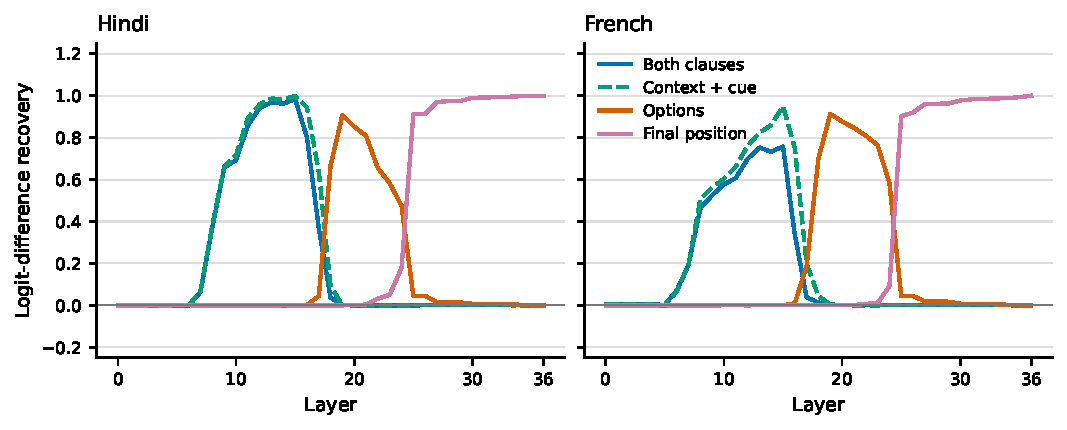
\includegraphics[width=\textwidth]{fig/e2_route.pdf}
\caption{Recovery from minimal-partner residual-stream patches across layers (96 pairs per language). Recovery normalizes the change in mean answer logit difference by the difference between partner and recipient (Equation~\ref{eq:recovery}). Both clauses excludes the negation cue; context includes it.}
\label{fig:heat}
\end{figure*}

Donor controls help distinguish the information associated with these sites. A context donor with different names and objects still recovers 0.95 in Hindi and 0.86 in French at layer 15. When the donor's option order is also reversed, context recovery remains 1.00 and 0.95, whereas option recovery at layer 19 falls to 0.07 and 0.11. Thus, the context effect is robust to these lexical and option-order changes, while the later option effect depends strongly on the answer mapping. Further interventions on question polarity and exchanged context names support the view that information about the named person and the question reaches the options before the final answer is selected. They do not by themselves prove a single serial path or specify every computation along it.

The individual donor comparisons give a more detailed ordering. With the context names exchanged, an option-group patch at layer 14 recovers 0.80 / 0.98 (Hindi / French). Changing question polarity gives recovery of 0.54 / 0.71 at the question tokens at layer 15, and patching the question and options together recovers 0.94 in both languages at layer 17. With the minimal partner, option A alone at layer 19 recovers 0.36 / 0.39, less than the two-option group. These comparisons support the presence of person, question and answer-relevant information at different sites, but their differing donors are not independent measurements of a single variable.

Groups of attention heads contribute to the option and final-position effects (Table~\ref{tab:heads}). Heads were ranked on 32 discovery pairs and first evaluated on 32 other discovery pairs; the selected sets were then evaluated on 64 test pairs. The top eight option-stage heads recover 0.89 in Hindi and 0.79 in French on test, and seven head identities overlap across the two languages. Resampling these outputs from items with the opposite negated mention reduces accuracy to 0.00 and 0.13, respectively; random sets of eight heads do not have this effect. The analogous final-position set also has a strong patching effect. These results support a concentrated causal contribution from the selected groups in this task; they do not show that each head has a separate, interpretable role.

The intermediate formatting tokens show a less concentrated effect: the top eight heads in layers 19--24 recover 0.49 / 0.58 on test, whereas the corresponding resampling accuracies are 0.60 / 0.57. In an attention-pattern analysis, L13H13 assigns 0.98 versus 0.01 of its attention to the option person's clause versus the other clause in Hindi (0.89 versus 0.04 in French). The pattern is consistent with person-specific lookup, although attention weights alone do not establish that the head transmits polarity. The full head-set controls and shared identities are in Appendix~\ref{app:heads}.

\begin{table}[t]
\small\centering
\begin{tabularx}{\linewidth}{@{}Xcc@{}}
\toprule
 & Options & Final position \\
Layers & 16--19 & 23--26 \\
\midrule
Top 8: partner recovery & .89 / .79 & .85 / .85 \\
Random 8: partner recovery & .00 / .00 & $-$.01 / $-$.01 \\
Top 8: resampled accuracy & .00 / .13 & .00 / .00 \\
Random 8: resampled accuracy & 1.00 / 1.00 & 1.00 / 1.00 \\
\bottomrule
\end{tabularx}
\caption{Head-set interventions on 64 held-out pairs, Hindi / French. Resampling uses an item with the opposite negated mention, matched on family, question polarity, and option order. Random-head results average five draws.}
\label{tab:heads}
\end{table}

A separate mean-ablation analysis tested whether late heads favor the affirmative person, as suggested by an English negation study \citep{zhou2026negation}. Across the 512 heads in layers 20--35, no individual head showed the predicted opposite effects on affirmative and negative questions. The effects across the two question types correlate at 0.99 in both languages. This negative result concerns this intervention and task; it does not rule out such heads in other models or prompts.

\subsection{Candidate variables and cross-lingual transfer}
\label{sec:subspaces}
The subspace interventions are consistent with a change in the information most effective at successive sites (Table~\ref{tab:das}). For clause tokens at layer 14, the $W$ intervention attains mean interchange accuracy of 0.88 in Hindi and 0.82 in French across three seeds. At the final position in layer 27, the answer-letter intervention attains 1.00 in both languages. Random subspaces score 0.00 at the tested sites. Some alternative variables also have substantial effects at option tokens, so the results should not be read as proof that each site stores exactly one variable.

\begin{table}[t]
\small\centering
\begin{tabularx}{\linewidth}{@{}Xcc@{}}
\toprule
Site and candidate & Within language & Cross-language \\
\midrule
Clauses L14, $W$ & .88 / .82 & .09 / .53 \\
Options L18, $Z$ & .65 / .83 & .52 / .38 \\
Options L19, \textbf{ANS} & .93 / .98 & .96 / .57 \\
Final L27, \textbf{ANS} & 1.00 / 1.00 & 1.00 / .99 \\
\bottomrule
\end{tabularx}
\caption{Interchange accuracy, averaged over three seeds. Within-language columns are Hindi / French; cross-language columns are Hindi-trained on French / French-trained on Hindi. Each test uses a frozen eight-dimensional basis and pairs differing in the target variable.}
\label{tab:das}
\end{table}

Transfer is much stronger at the final answer position than at the clause site. The Hindi-trained $W$ subspace achieves 0.09 on French, and the French-trained one achieves 0.53 on Hindi, compared with 1.00 and 0.99 for the final answer subspaces. This asymmetry is not proof that clause representations are wholly language-specific: the learned subspaces are non-unique, token alignment differs between languages, and a jointly trained subspace achieves mean $W$ accuracy of 0.75 on Hindi and 0.63 on French over two seeds. Rather, the comparison indicates that the independently learned clause directions transfer less reliably under this procedure than the answer directions.

Cross-language sources further separate reading a direction from using it in a base. For $W$ at layer 14, a French-trained basis with a French base and Hindi source reaches 0.83 mean interchange accuracy, compared with 0.38 for the reverse arrangement using the Hindi-trained basis; these are means over three seeds. The jointly trained basis reaches 0.92 with a French base and Hindi source and 0.57 in the reverse direction, averaged over two seeds. These asymmetric interventions suggest partial alignment, but do not show that either language's entire representation is contained in the other's. Appendix~\ref{app:das} reports seed ranges and the corresponding within-language controls.

A dimensionality comparison also distinguishes these sites. A one-dimensional answer subspace at the final position attains 1.00 interchange accuracy in both languages; at the options it attains 0.81 / 0.96. For $W$ in the clauses, one dimension gives 0.59 / 0.23 and four give 0.72 / 0.74. These are particular learned subspaces, not estimates of the intrinsic dimension of a unique representation.

\subsection{Beyond a single negated mention}
\label{sec:generalization}
The base task always has one negated mention, so $W$ alone can identify both polarities. In explicit worlds we instead vary the polarity of each fact. With two people and two predicates, patching a donor that differs in the queried fact affects the answer, while changes to a different fact have effects below 0.04 across the tested layers and positions (64 pairs per language). A single learned basis applied at fact-token positions also changes target answers while leaving answers about other facts correct at rates of at least 0.96 in the reported runs. Target accuracy varies substantially across seeds: for Hindi two-predicate worlds it is 0.99 and 0.65 for same-slot interventions. This selectivity supports a fact-sensitive account, but the seed variation limits the precision of the claim.

The intervention exchanges one learned subspace at the fact tokens after the person's name. For one-predicate worlds, same-slot / different-slot target accuracies are 0.91 / 0.87 in Hindi and 0.74 / 0.85 in French. For two-predicate worlds, the corresponding two-seed means are 0.82 / 0.79 and 0.62 / 0.60. Other-fact accuracy remains high in these tests. Thus, the effect is not restricted to exchanging the same input position, but incomplete and seed-sensitive target control precludes claiming a perfectly localized fact variable.

\paragraph{Other forms and nested negation.} Late option and final-position patches remain effective across the six tested alternative form sets: layer-20 option recovery ranges from 0.79 to 0.91, and layer-26 final-position recovery from 0.87 to 0.93. In contrast, clause-group recovery at layer 14 varies from 0.04 to 0.98 across forms and languages. This contrast suggests that the tested late answer route is more stable than the early localization, although recovery can vary with donor and token alignment.

Frozen base-task subspaces show a similar qualification (Figure~\ref{fig:forms}). The clause-level $W$ subspace transfers to habitual negation and ``never'' at 0.63--0.95; for ``no longer'' it scores 0.90 in Hindi but 0.03 in French, and it fails on the tested lexical-negation condition in both. At the option site, answer-subspace transfer is 0.80--0.99 for forms other than focus; the final-position answer subspace transfers more broadly. The Hindi ``no longer'' template retains \hi{नहीं}, while the French cue changes from \emph{pas} to \emph{plus}; this surface difference is a possible explanation, not an isolated causal factor.

\begin{figure*}[t]
\centering
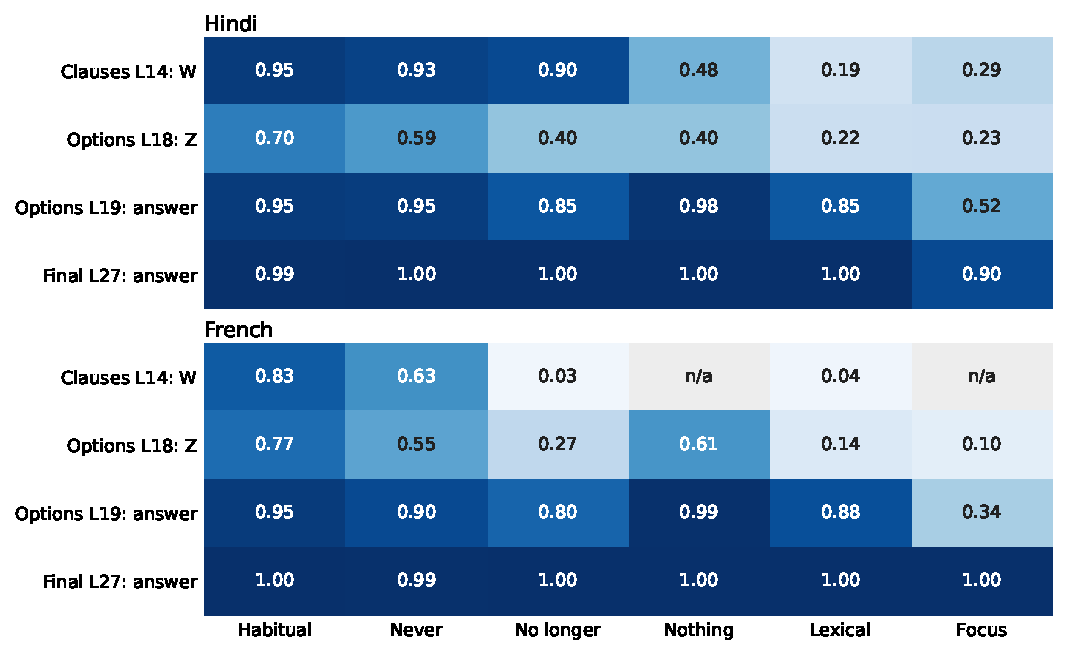
\includegraphics[width=\textwidth]{fig/e3_forms_readable.pdf}
\caption{Transfer to other negation forms of eight-dimensional subspaces learned on the base task. Cells give interchange accuracy by language, site, and candidate variable; n/a indicates that the necessary role was unavailable. These are single-seed evaluations and should be interpreted alongside the seed variation for the base task.}
\label{fig:forms}
\end{figure*}

For nested negation, we compare causal models that interchange either the inner fact's polarity or its composed polarity. On examples where these models predict different answers, the inner-polarity model fits better at Hindi layers 11 and 13, while the composed-polarity model fits better at French layer 13. Both outcomes recur across two seeds, with variable strengths (Appendix~\ref{app:worlds}); they characterize particular sites, not the full computation of nested scope.

The exception results expose a behavioral limit that perfect base accuracy conceals. For the Hindi wording corresponding to ``nobody except X likes curd,'' the model frequently answers that a non-exception person likes it. In a 500-item-per-wording follow-up analysis, accuracy for other people varies from 14\% to 67\% across three Hindi exception markers, and rises to 100\% for one marker when the exception follows the negative sentence. Equivalent statements using ``only'' or two sentences also reach 100\%. In French, moving \emph{sauf X} before \emph{personne} reduces accuracy on questions about X from 98\% to 46\%. Word order and wording are associated with the errors (Table~\ref{tab:except}), but these comparisons do not isolate their causal mechanism; the conditions also change the surface form and may vary in naturalness.

The converse quantifier exposes another failure. For Hindi ``everyone except X'' with \hi{के सिवा}, accuracy on X is 3\% when the exception comes first and 13\% when it follows, even though accuracy on other people is 96\% and 88\%. French reaches approximately 100\% for this condition in either order. The full 500-item wording comparisons, including counts by question target, are in Appendix~\ref{app:exceptions}.

\paragraph{Patching quantifiers and exceptions.} We also intervene on the successful quantifier conditions, contrasting matched ``everyone'' and ``nobody'' sentences (24 pairs per condition and language). The question tokens recover 0.47 / 0.44 at layer 16, the option group recovers 0.95 / 0.94 at layer 20, and the final position becomes effective from layer 26. With an exception present in both donor and recipient, French \emph{sauf} follows the quantifier and its token recovers 0.85--0.94 at layers 12--14. The Hindi exception phrase precedes the quantifier and its patch has approximately zero recovery, while the whole sentence recovers 0.66--0.86 for questions about the exception. The positional contrast is compatible with the autoregressive ordering of these cues; differences in wording, tokenization, and the patch site prevent a causal attribution to word order alone.

\begin{table}[t]
\small\centering
\begin{tabularx}{\linewidth}{@{}Xrr@{}}
\toprule
``Nobody except X'' wording & X & Other \\
\midrule
Hindi: X \hi{को छोड़कर}, before & 95 & 14 \\
Hindi: X \hi{के अलावा}, before & 89 & 67 \\
Hindi: X \hi{के सिवा}, before & 98 & 57 \\
Hindi: X \hi{के सिवा}, after & 100 & 100 \\
Hindi: ``only X'' & 100 & 100 \\
French: \emph{sauf X}, after & 98 & 100 \\
French: \emph{sauf X}, before & 46 & 100 \\
\bottomrule
\end{tabularx}
\caption{Accuracy (\%) on 500 items per wording, split between questions about the exception (252) and another person (248); columns give accuracy by question target. ``Before'' and ``after'' indicate the position of the exception phrase relative to the quantified clause.}
\label{tab:except}
\end{table}

\subsection{What an activation oracle can read}
\label{sec:oracle}
We query a released Qwen3-4B activation oracle \citep{karvonen2026oracles} with English yes/no questions about activations from 300 test items per language. On clause-one tokens at layer 18, it answers whether the person has the relevant property with 0.99 / 1.00 accuracy (Hindi / French). On the option-A name at the same layer, accuracy is 0.66 / 0.57; on the full context, the question of whether the first mention is negated yields 0.50 / 0.50. A linear probe trained on a random half of the same sampled activations reaches 1.00 on the corresponding held-out half. The comparison shows that information can be linearly recoverable without being reliably elicited by this oracle and wording; the two methods differ in training and evaluation and are not directly equivalent (Table~\ref{tab:oracle}).

\begin{table}[t]
\small\centering
\begin{tabularx}{\linewidth}{@{}Xcc@{}}
\toprule
Question and activation & Oracle & Adapter off \\
\midrule
Person's polarity, clause 1, L18 & .99 / 1.00 & .57 / .64 \\
First mention negated, context, L18 & .50 / .50 & .50 / .50 \\
Person's polarity, option A, L18 & .66 / .57 & .42 / .43 \\
Answer is A, final position, L27 & .95 / .96 & .55 / .54 \\
\bottomrule
\end{tabularx}
\caption{Oracle accuracy on 300 sampled test items per language (Hindi / French), compared with activation injection with the adapter disabled. A linear probe trained and evaluated on separate random halves of the same samples reaches 1.00 in each row.}
\label{tab:oracle}
\end{table}

At layer 27 the oracle predicts whether A is correct at 0.95 / 0.96 accuracy. After clause-group patching at layer 13, it agrees with the patched model's answer on 0.94 / 0.93 of 96 pairs. Agreement falls to 0.76 / 0.92 after an option-group patch. These interventions show that the readout often tracks changes in the model's answer, while also exposing a failure mode for one patch and language.

Agreement alone can be misleading when the intervention leaves the model's answer unchanged. For the two-clause patch, the model's answer changes on 100\% / 73\% of the pairs; for the option patch it changes on 98\% / 95\%. Single-clause patches change at most 10\%, despite high oracle--model agreement. Appendix~\ref{app:oracle} reports both quantities for each condition, so that agreement is not mistaken for an intervention success rate.

\section{Discussion and conclusion}
\label{sec:discussion}
The central contrast is between the early and late stages of the tested computation. Clause-group patches carry information that changes the answer even with different names and objects, but independently learned clause subspaces transfer unevenly between languages. At the final position, answer-letter subspaces transfer nearly perfectly in both directions. Together with the overlap in influential head sets, these findings are consistent with some shared answer-selection machinery following more variable processing of the linguistic input. They do not establish that all languages or all negation constructions converge on the same mechanism.

The fact-level experiments and exception errors qualify that account. Interventions in explicit worlds can selectively affect a queried fact, but their strength varies across optimization seeds. The exception tests show that a model can perform perfectly on simple balanced pairs while failing on a particular quantifier construction. A useful next step is to validate the templates with fluent speakers and test whether the same patterns persist in naturalistic text and additional model families.

\section*{Limitations}
The main causal analysis concerns one model, two languages, and synthetic templates; it does not establish general behavior in other models or natural settings. The two languages also differ in script, tokenization, and word order, preventing us from attributing transfer differences to any one linguistic feature. Not all extended templates have been checked by fluent speakers, and some exception word orders may differ in naturalness. Head sets were selected using small discovery samples, and many analyses use 24--96 intervention pairs. Main subspace results use three seeds; several extended analyses use only one or two. Activation patching can introduce out-of-distribution states, and low recovery from one position does not exclude redundant or distributed information. Finally, the oracle and linear probe use different training procedures, so their accuracies should not be treated as a controlled comparison of intrinsic representational content.

\bibliography{refs}

\clearpage
\appendix
\section{Task inventory and reproducibility}
\label{app:data}
Table~\ref{tab:taskinventory} summarizes the constructed task families. In the base task, the discovery, development and test files contain 48,640, 5,760 and 12,960 negative examples, respectively, plus 2,000, 500 and 500 affirmative controls per language. The split is by names and objects; the ability family occurs only in test. Base-task partner interventions use preference and possession examples, as the patching sampler explicitly restricts these families. The extended sets vary the wording and answer format, so a high base-task score alone does not validate every intervention condition.

\begin{table}[t]
\small
\begin{tabularx}{\linewidth}{@{}lX@{}}
\toprule
Set & Construction \\
\midrule
Habitual & Negated and affirmative habitual activities \\
Never & \emph{ne ... jamais} / Hindi ``never'' with negation \\
No longer & Past context followed by current negative state \\
Nothing & Negative indefinite contrasted with an affirmative fact \\
Lexical & Lexically negative versus explicitly negated predicates \\
Focus & Negation contrasts two objects or two people \\
Quantifiers & Everyone or nobody, with or without an exception; ``not everyone'' \\
One-predicate worlds & Two people, four polarity configurations \\
Two-predicate worlds & Two people and two predicates, sixteen configurations \\
Nested & An outer negation around a queried fact \\
\bottomrule
\end{tabularx}
\caption{Extended task families. The first six use name or object answer options; the remaining sets use yes/no options. Examples and generator details are in \texttt{data/templates.md}.}
\label{tab:taskinventory}
\end{table}

All experiments use the model and data files named in the repository. In the default base-task DAS script, the same basis is applied at each aligned token in a selected role group; bases are optimized with Adam and binary cross-entropy on the A/B logit difference. Learning rates, batch sizes, steps and evaluation sample counts vary across runs and seeds, and the executed configurations are recorded in \texttt{jobs/cmds/} and result-file metadata. The primary seed checks use 200 evaluation pairs per seed for the additional seed runs; runs should be compared using their stored arguments rather than assuming identical optimization budgets. For full-model inference we used one RTX 2080 Ti. The released oracle adapter reads layers 9, 18 and 27; its activations are injected into the adapter's input at placeholders, and answers are scored using Yes/No logits.

\paragraph{Smaller model.} Qwen3-1.7B scores 49--69\% in zero-shot Hindi across the base families, versus 96--100\% in French. Two fixed examples raise its Hindi result to approximately 99\%. With zero-shot French, residual patching shows a qualitatively similar sequence at earlier layers: context through layer 11 (0.74 recovery), options at layers 14--15 (0.97), and the final position from layer 22. This is a limited comparison, not a replication of every 4B experiment.

\section{Head and donor controls}
\label{app:heads}
Table~\ref{tab:appendixheads} includes the intermediate label/template destination omitted from the condensed main-text table. All sets contain eight heads and were chosen on discovery data. On the 32-pair discovery evaluation, the option-stage top eight recover 0.90 / 0.88 while the remaining 120 heads in the same four layers recover 0.03 / 0.05. The best single head recovers 0.02 / 0.04. Joint effects and redundancy make these quantities non-additive.

\begin{table}[t]
\small\centering
\begin{tabularx}{\linewidth}{@{}Xccc@{}}
\toprule
 & Options & Label & Final \\
Layers & 16--19 & 19--24 & 23--26 \\
\midrule
Partner patch: top 8 & .89 / .79 & .49 / .58 & .85 / .85 \\
Partner patch: random 8 & .00 / .00 & .00 / .00 & $-$.01 / $-$.01 \\
Resample: top 8 & .00 / .13 & .60 / .57 & .00 / .00 \\
Resample: random 8 & 1.00 / 1.00 & 1.00 / 1.00 & 1.00 / 1.00 \\
\bottomrule
\end{tabularx}
\caption{Test-split head controls (64 pairs; Hindi / French). Rows report recovery for partner patches and accuracy for resampling from a different item with the opposite negated mention. Random results average five draws. The label group includes ``B:'' and chat-template tokens.}
\label{tab:appendixheads}
\end{table}

The seven heads common to the Hindi and French option-stage top-eight sets are L16H17, L17H4, L18H8, L18H11, L18H15, L19H10 and L19H31; six of the eight final-position heads overlap. Resampling the selected sets from another item with the \emph{same} negated mention retains 0.99--1.00 of the clean logit difference. For late mean ablations, the largest difference between effects on affirmative and negative questions is 0.51 in Hindi and 0.61 in French. L34H29 opposes the correct answer under both question polarities, so its effect alone is not evidence of an affirmative-person shortcut.

\section{Subspace transfer and seed variation}
\label{app:das}
Table~\ref{tab:seedrange} reports the range behind the three-seed means in the main text. The range at the intermediate option site is wider than at the final position. Applying a frozen basis trained in one language to both base and source examples in another tests a different condition from holding the base language fixed while changing the source language. We report both rather than treating them as interchangeable evidence of cross-language alignment.

\begin{table}[t]
\small\centering
\begin{tabularx}{\linewidth}{@{}Xcc@{}}
\toprule
Site / variable & Hi $\rightarrow$ Fr & Fr $\rightarrow$ Hi \\
\midrule
Clauses L14, $W$ & .05--.11 & .49--.56 \\
Options L18, $Z$ & .37--.61 & .33--.41 \\
Options L19, \textbf{ANS} & .90--.99 & .45--.77 \\
Final L27, \textbf{ANS} & 1.00 & .97--1.00 \\
\bottomrule
\end{tabularx}
\caption{Ranges of cross-language interchange accuracy over three seeds. The arrow indicates the training language followed by the language of both test activations.}
\label{tab:seedrange}
\end{table}

The first-seed within-language grid (Table~\ref{tab:allvars}) compares all three candidate variables at each principal site. Only the principal candidate at each site is summarized across seeds in Table~\ref{tab:das}; the other grid cells are single-seed results. Cross-variable effects, especially at the option site, are one reason not to treat the candidate variables as uniquely localized.

\begin{table}[t]
\small\centering
\begin{tabularx}{\linewidth}{@{}Xccc@{}}
\toprule
Site & $W$ & $Z$ & \textbf{ANS} \\
\midrule
Clauses L14 & .92 / .81 & .17 / .03 & .33 / .09 \\
Options L18 & .07 / .25 & .75 / .90 & .23 / .66 \\
Options L19 & .12 / .34 & .60 / .56 & .93 / .97 \\
Final L27 & .01 / .10 & .38 / .45 & 1.00 / 1.00 \\
\bottomrule
\end{tabularx}
\caption{First-seed within-language interchange accuracy for each candidate variable and site, Hindi / French. Three-seed means for the principal candidate at each site appear in Table~\ref{tab:das}.}
\label{tab:allvars}
\end{table}

With a French-trained clause basis, a French base and Hindi source yield 0.83 mean accuracy (range 0.79--0.91), close to the French within-language mean of 0.82. With a Hindi-trained basis, a Hindi base and French source yield 0.38 (0.34--0.43), below its Hindi within-language mean of 0.88. The jointly trained eight-dimensional basis scores 0.77 / 0.72 on Hindi and 0.54 / 0.72 on French across its two seeds. These results allow a shared-direction interpretation but do not demonstrate identical distributions of the full hidden states.

For affirmative controls, the $W$ and $Z$ interventions at their principal sites preserve the base answer at 0.99--1.00. The answer-letter intervention changes it on about half of these controls, consistent with a letter-level rather than negation-specific intervention. Random bases of the same size score 0.00 on the selected different-variable pairs.

\section{Fact-level and nested-polarity interventions}
\label{app:worlds}
For two people and two predicates, Table~\ref{tab:worldseeds} reports accuracy when the intervention should change the queried fact and when it should leave a different fact unchanged. The same learned basis is applied to every fact slot; ``same'' and ``different'' identify the relation between the recipient and donor fact indices. High other-fact accuracy is an observed selectivity measure, conditional on this intervention and these questions.

\begin{table}[t]
\small\centering
\begin{tabularx}{\linewidth}{@{}Xccc@{}}
\toprule
Language, layer, seed & Same & Different & Other \\
\midrule
Hindi L13, seed 0 & .99 & .97 & .99 \\
Hindi L13, seed 1 & .65 & .61 & .98--.99 \\
French L15, seed 0 & .62 & .54 & .97--.98 \\
French L15, seed 1 & .62 & .65 & .96 \\
\bottomrule
\end{tabularx}
\caption{Two-predicate world interventions. Same / different are target interchange accuracies for matching / differing fact slots. Other is the range of accuracies for questions about unmodified facts across these slot conditions.}
\label{tab:worldseeds}
\end{table}

For nested items we score only cases where the inner and composed models predict different answers. At Hindi layer 11, inner-polarity accuracy is 0.99 / 0.77 across seeds versus 0.45 / 0.32 for composed polarity. At French layer 13, inner accuracy is 0.64 / 0.72 versus 0.91 / 0.89 for composed polarity. These are separate learned intervention models, not direct measurements of a single scalar code.

\section{Exception wording and question targets}
\label{app:exceptions}
Table~\ref{tab:fullexceptions} gives both quantifier conditions. Each wording uses 500 examples: 252 questions about X and 248 about a different person. The original dataset evaluation reports 12.9\% accuracy for non-exception questions, while the wording-analysis rerun reports 13.7\% (rounded to 14\%) on the same 248 base-condition items. The saved runs do not establish the reason for this small discrepancy; we retain the values reported by each run.

\begin{table}[t]
\small\centering
\begin{tabularx}{\linewidth}{@{}Xcc@{}}
\toprule
Wording & Nobody & Everyone \\
 & X / other & X / other \\
\midrule
Hindi \hi{को छोड़कर}, before & 95 / 14 & 100 / 98 \\
Hindi \hi{के अलावा}, before & 89 / 67 & 89 / 97 \\
Hindi \hi{के सिवा}, before & 98 / 57 & 3 / 96 \\
Hindi \hi{को छोड़कर}, after & 79 / 57 & 84 / 94 \\
Hindi \hi{के सिवा}, after & 100 / 100 & 13 / 88 \\
Hindi ``only X'' & 100 / 100 & -- \\
Hindi two sentences & 100 / 100 & -- \\
French \emph{sauf X}, after & 98 / 100 & 100 / 100 \\
French \emph{sauf X}, before & 46 / 100 & 100 / 100 \\
\bottomrule
\end{tabularx}
\caption{Accuracy (\%) by quantifier, wording and target of the question. Before / after denotes the exception phrase's position relative to the quantified clause. ``Nobody'' and ``Everyone'' mean the respective quantifier with an exception. Values are rounded.}
\label{tab:fullexceptions}
\end{table}

\section{Oracle behavior after interventions}
\label{app:oracle}
Table~\ref{tab:oraclepatch} separates the model answer-change rate from oracle--model agreement. The oracle reads the final-position layer-27 state after each intervention, so unchanged answers contribute to agreement as well as changed answers. These aggregates therefore do not separately measure oracle accuracy on only the changed subset.

\begin{table}[t]
\small\centering
\begin{tabularx}{\linewidth}{@{}Xcc@{}}
\toprule
Patch & Answer changed & Agreement \\
\midrule
None & .00 / .00 & .94 / .95 \\
Both clauses, L13 & 1.00 / .73 & .94 / .93 \\
Clause 1, L13 & .01 / .04 & .92 / .97 \\
Clause 2, L13 & .10 / .07 & .91 / .95 \\
Options, L19 & .98 / .95 & .76 / .92 \\
\bottomrule
\end{tabularx}
\caption{Model answer-change rate and oracle agreement with the patched model on 96 pairs, Hindi / French. Agreement is over all pairs.}
\label{tab:oraclepatch}
\end{table}

\end{document}
